\documentclass[../note.tex]{subfiles}
\usepackage{bm}

\begin{document}


\chapter{Bayesian Filter}

\section{Basic Settings}

Let 
\[
    \bm{x}_t \in \mathbb{R}^{n_{\bm{x}}}
\]
denote the state vector at time $t$, which represents the unknow quantity we want to infer.

At each time $t$, we observe 
\[
    \bm{z}_t \in \mathbb{R}^{n_{\bm{z}}}.
\]
The observation contains information about the hidden state $\bm{x}_t$, but may be noisy and uncertain. For convenience, deine the observation history up to time $t$ as
\[
    \bm{z}_{1:t} = \left\{ \bm{z}_1, \dots, \bm{z}_t \right\}
\]

Similarly, suppose that a control input is available at each time $t$, denoted by
\[
    \bm{u}_t \in \mathbb{R}^{n_{\bm{u}}},
\]
with the corresponding control history 
\[
    \bm{u}_{1:t} = \left\{ \bm{u}_1, \dots, \bm{u}_t \right\}.
\] 

Therefore, the available information evolves sequentially as
\[
    \bm{u}_1, \bm{z}_1, \bm{u}_2, \bm{z}_2, \bm{u}_3, \bm{z}_3, \dots
\]
whereas the states
\[
    \bm{x}_1, \bm{x}_2, \dots.
\]
are not directly observed.

Since subsequent inference depends on the state, the objective is to characterize the uncertainty associated with the random variable $\bm{x}_t$ given all available information. This uncertainty is represented by the belief state
\[
    \mathrm{bel}(\bm{x}_t) = p(\bm{x}_t | \bm{z}_{1:t}, \bm{u}_{1:t}).
\]
The belief state is therefore a probability distribution over the possible values of $\bm{x}_t$ conditioned on the available observation and control histories. It is also commonly referred to as the posterior state distribution, information state, or state of knowledge. 


\section{Bayesian Filter Derivation}

The key idea of Bayesian filter is to represent uncertainty explicitly using the calculas of probability theory. 

At each time step, the hidden state $\bm{x}_t$ evolves from the previous state $\bm{x}_{t-1}$ under the control input $\bm{u}_t$, while the observation $\bm{z}_t$ is generated from the corresponding state $\bm{x}_t$, as shown in Figure~\ref{fig-1}.
\begin{figure}[H]
    \centering
    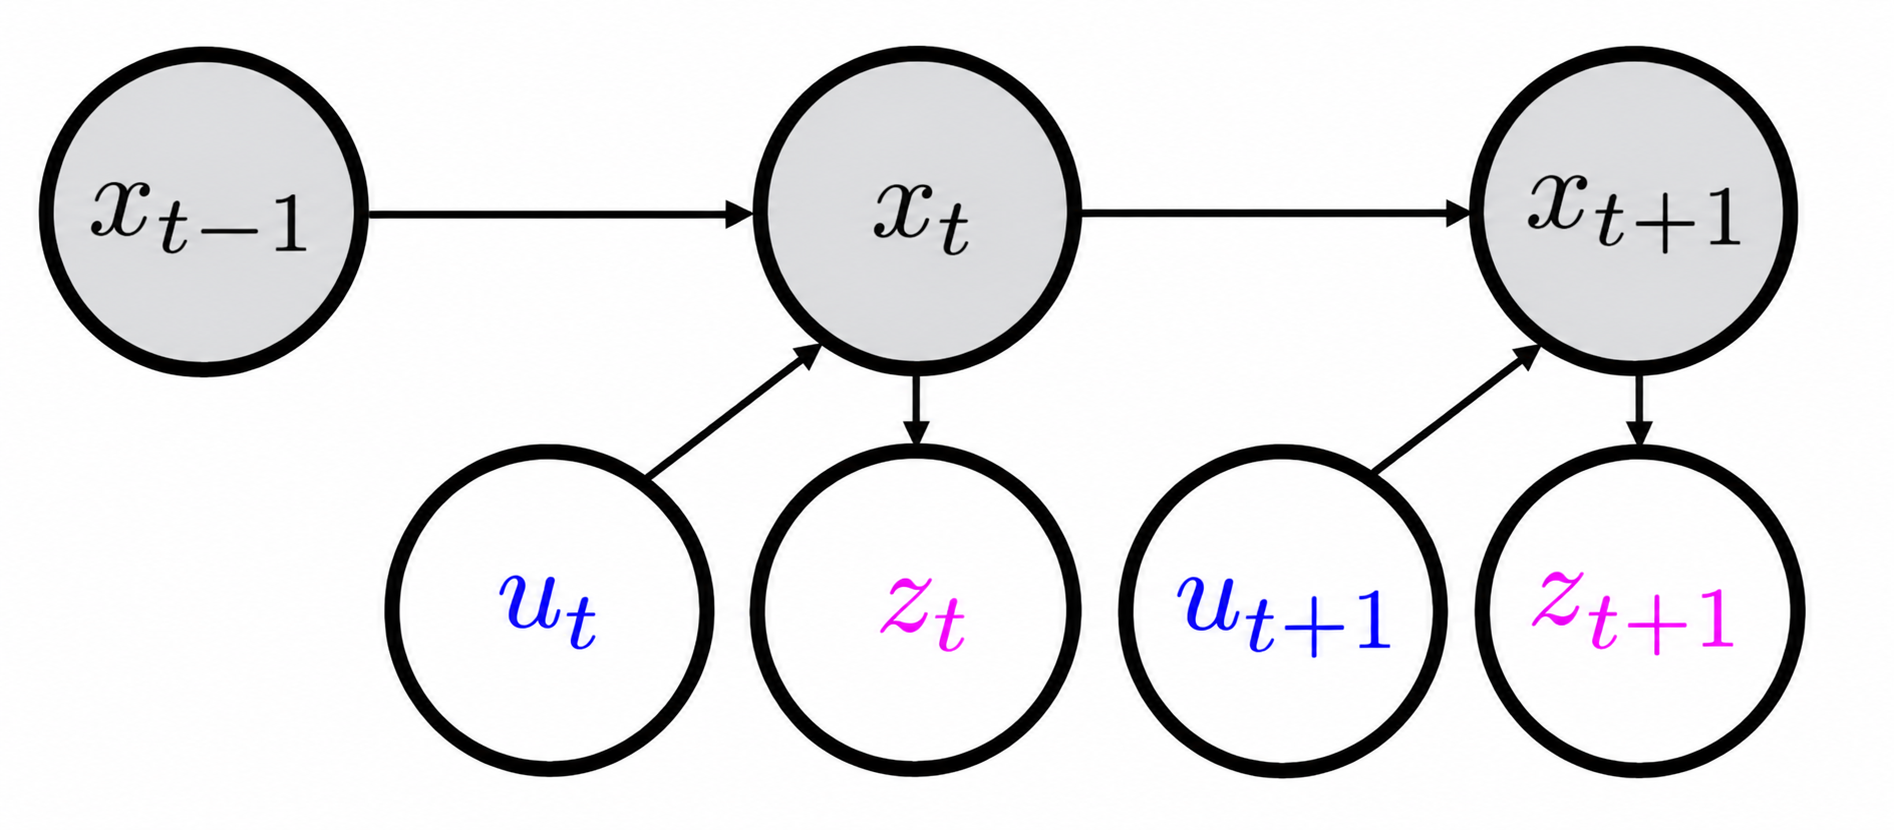
\includegraphics[width=0.4\textwidth]{fig-1.png}
    \caption{Graphical representation of the Bayesian filtering model}
    \label{fig-1}
\end{figure}

However, the belief, $p(\text{current sate} | \text{all past information})$, is intractable. This leads to the Markov assumption: future state conditionally independent of past control inputs and observations given present state. We therefore have
\[
    \begin{aligned}
        & p(\bm{x}_t | \bm{x}_{t-1}, \bm{u}_t, \bm{z}_{1:t-1}, \bm{u}_{1:t-1}) = p(\bm{x}_t | \bm{x}_{t-1}, \bm{u}_t), \\
        & p(\bm{z}_t | \bm{x}_{t}, \bm{u}_t, \bm{z}_{1:t-1}, \bm{u}_{1:t-1}) = p(\bm{z}_t | \bm{x}_{t}).
    \end{aligned}
\]

Using Bayes' rule and the Markov assumptions,
\[
    \begin{aligned}
        \mathrm{bel}(\bm{x}_t) & = p(\bm{x}_t | \bm{z}_{1:t}, \bm{u}_{1:t}) = p(\bm{x}_t | \bm{z}_t, \bm{u}_t, \bm{z}_{1:t-1}, \bm{u}_{1:t-1}) \\
        & = \frac{p(\bm{x}_t, \bm{z}_t | \bm{u}_t, \bm{z}_{1:t-1}, \bm{u}_{1:t-1})}{p(\bm{z}_t | \bm{u}_t)} \leftarrow \text{Condition probability} \\
        & = \eta p(\bm{x}_t, \bm{z}_t | \bm{u}_t, \bm{z}_{1:t-1}, \bm{u}_{1:t-1}) \leftarrow \text{Normalization constant}\\
        & = \eta p(\bm{z}_t | \bm{x}_t, \bm{u}_t, \bm{z}_{1:t-1}, \bm{u}_{1:t-1}) p(\bm{x}_t | \bm{u}_t, \bm{z}_{1:t-1}, \bm{u}_{1:t-1}) \leftarrow \text{Bayes rule}  \\
        & = \eta p(\bm{z}_t | \bm{x}_t) p(\bm{x}_t | \bm{u}_t, \bm{z}_{1:t-1}, \bm{u}_{1:t-1}) \leftarrow \text{Markov assumption}  \\
        & = \eta p(\bm{z}_t | \bm{x}_t) \int p(\bm{x}_t, \bm{x}_{t-1} | \bm{u}_t, \bm{z}_{1:t-1}, \bm{u}_{1:t-1}) \mathrm{d} x_{t-1} \leftarrow \text{Opposite of marginalization} \\
        & = \eta p(\bm{z}_t | \bm{x}_t) \int p(\bm{x}_t  | \bm{x}_{t-1}, \bm{u}_t, \bm{z}_{1:t-1}, \bm{u}_{1:t-1}) p (\bm{x}_{t-1} | \bm{u}_t, \bm{z}_{1:t-1}, \bm{u}_{1:t-1}) \mathrm{d} x_{t-1} \leftarrow \text{Probability chain rule} \\
        & = \underbrace{\eta p(\bm{z}_t | \bm{x}_t)}_{\text{correction}}  \underbrace{\int p(\bm{x}_t  | \bm{x}_{t-1}, \bm{u}_t) \mathrm{bel}(\bm{x}_{t-1}) \mathrm{d} x_{t-1}}_{\text{prediction}}
    \end{aligned} 
\]
where $\eta$ is a normalization constant and $\eta = \frac{1}{p(\bm{z}_t | \bm{u}_t)}$ and $\mathrm{bel}(x_0)$ = $p(\bm{x}_0)$.

Bayesian filter therefore provides a recursive update approach to calculate belief tractably consisting of two steps: prediction, which propagates the previous belief through the motion model, and correction, which incorporates the latest observation through the measurement model.


\end{document}